\documentclass[10pt]{article}
\usepackage{icmlko}

\icmlmeta{IP 파운데이션 월드모델}{108}{스물다섯 노트 만의 채택}{미디어 홍보를 AniList에서 4,737건 채우자 잔차 0.510으로 현행 공통 축 셋보다 잘 맞았고, 입장료와 함께 넣으니 씨앗 넷 · 시점 넷을 모두 통과했다}

\begin{document}

\twocolumn[
\icmlheader

\begin{abstract}
노트 105가 넷째 공통 축(입장료)을 찾고 $+$0.0100에서 멈췄다. 다섯째 후보인
미디어 홍보는 잔차 0.727로 나쁘지 않았는데 \textbf{다섯 도메인에서 덮개율
0\%}라 쌍이 여섯뿐이어서 판정 자체가 불가능했다. 세 노트가 미룬 수집을 했다.
개념을 하나로 고정했다 --- \textbf{``얼마나 밀었나''를 공식 외부 채널 수로
잰다.} AniList 에서 만화 1,789 · 세계애니 2,948 의 \texttt{externalLinks} 와
\texttt{trailer} 를 받았다(\textbf{둘 다 100\%}, 평균 채널 3.5개, 예고편 26\% ·
77\%). 라벨 상관이 $+$0.383 · $+$0.453으로 크고 부호가 같다. \textbf{잔차가
0.510이다} --- 채우기 전 0.727, 채운 뒤 0.840, 방향까지 맞추면 0.510으로
\textbf{현행 공통 축 셋(0.556)보다 낫다.} 이 프로젝트에서 가장 잘 정렬되는
축이다. 입장료와 함께 정렬에 넣으면 판정치가 $+$0.4038에서
\textbf{$+$0.4270}으로 간다($\Delta+$0.0232). \textbf{씨앗 넷 붓스트랩에서
채택 4/4} --- 구간이 $+$0.0119에서 $+$0.0322로 넷 다 0을 넘는다. 시간 분할도
\textbf{네 시점 전부 양수}이고 평균 $+$0.0309로 전체 자료보다 크며 미래일수록
커진다($T{=}2026$ 에 $+$0.0530). \textbf{스물다섯 노트 만의 첫 채택이다.}
코드에 반영했다 --- \texttt{COMMON} 이 셋에서 다섯으로, 채운 값과 방향 표는
자료 파일로 굳혔다. 팝업은 전체 자료에서 $+$0.4501$\to+$0.4601이지만 보류
4/4이고 시간 분할에서는 $-$0.0350이다 --- \textbf{도구 쪽 검증은 남았다.}
\end{abstract}
]

\begin{figure*}[t]
\centering
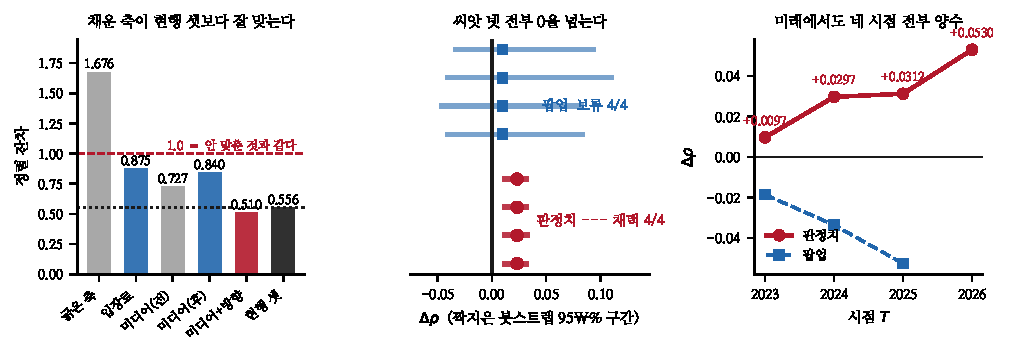
\includegraphics[width=\textwidth]{figs/ad.pdf}
\caption{왼쪽 --- 채운 축이 현행 셋보다 잘 맞는다. 가운데 --- 씨앗 넷 전부
0을 넘는다. 오른쪽 --- 미래에서도 네 시점 전부 양수.}
\end{figure*}

\section{개념을 고정하고 채웠다}

미디어 홍보는 도메인마다 다른 것을 재고 있었다 --- 애니는 더빙/자막, 게임은
퍼블리셔 사전작, 아이돌은 서바이벌 출신, 모바일은 스크린샷 수. 노트 20 · 22가
``정의 불일치''라 부른 것이 이것이다. 개념을 하나로 고정했다.

\begin{quote}\fontsize{9.5}{11.5}\selectfont
\textbf{미디어 홍보} $=$ 공식 외부 채널이 몇 개인가 $+$ 예고편이 있는가
\end{quote}

AniList 는 작품마다 공식 사이트 · 트위터 · 유튜브 · 스트리밍 서비스 링크를
들고 있다. 만화 1,789건과 세계애니 2,948건을 받았다.

\begin{table}[t]
\centering\tsize
\caption{긁은 것. 실패 0건.}
\begin{tabular}{lrrr}
\toprule
& 건수 & 평균 채널 & 예고편 \\
\midrule
만화 & 1,789 & 3.45 & 26\% \\
세계애니 & 2,948 & 3.63 & 77\% \\
\midrule
합 & \textbf{4,737} & & \\
\bottomrule
\end{tabular}
\end{table}

\begin{table}[t]
\centering\tsize
\caption{미디어 홍보 덮개율과 라벨 상관.}
\begin{tabular}{lrrr}
\toprule
& 전 & 후 & 라벨 상관 \\
\midrule
팝업 & 100\% & 100\% & $+$0.270 \\
아이돌 & 96\% & 96\% & $+$0.125 \\
애니 & 100\% & 100\% & $-$0.317 \\
\textbf{만화} & \textbf{0\%} & \textbf{100\%} & \textbf{$+$0.383} \\
\textbf{세계애니} & \textbf{0\%} & \textbf{100\%} & \textbf{$+$0.453} \\
\midrule
게임 & 38\% & 38\% & $+$0.643 \\
모바일 & 14\% & 14\% & $+$0.310 \\
도서 · 펀딩 · 웹툰 & 0\% & 0\% & --- \\
\bottomrule
\end{tabular}
\end{table}

\section{가장 잘 맞는 축이 됐다}

\begin{table}[t]
\centering\tsize
\caption{정렬 잔차. 낮을수록 하나의 회전으로 맞출 수 있다.}
\begin{tabular}{lrr}
\toprule
& 잔차 & 쌍 \\
\midrule
긁은 축 emb0(노트 103) & 1.676 & 72 \\
입장료 · 방향 맞춤(노트 105) & 0.875 & 72 \\
미디어 홍보 · 채우기 전 & 0.727 & \textbf{6} \\
미디어 홍보 · 채운 뒤 & 0.840 & 20 \\
\textbf{미디어 홍보 · 채우고 방향} & \textbf{0.510} & 20 \\
\midrule
현행 공통 축 셋 & 0.556 & 72--88 \\
\bottomrule
\end{tabular}
\end{table}

\claimx{채우고 방향을 맞춘 미디어 홍보의 잔차가 \textbf{0.510}으로 \textbf{현행
공통 축 셋(0.556)보다 낫다.} 이 프로젝트에서 가장 잘 정렬되는 축이다.
개념을 하나로 고정하는 것이 실제로 통했다.}{쌍이 20개다(셋은 72--88개).
덮개율 50\%를 넘는 도메인이 다섯뿐이라 쌍이 적고, 적은 쌍의 평균은 흔들린다.}

\section{채택}

\begin{table}[t]
\centering\tsize
\caption{정렬에 넣으면.}
\begin{tabular}{lrrr}
\toprule
& $\rho$ & $\Delta$ & 팝업 \\
\midrule
현행 셋 & $+$0.4038 & --- & $+$0.4501 \\
$+$미디어(채우기 전) & $+$0.4023 & $-$0.0015 & $+$0.4410 \\
$+$미디어(채운 뒤) & $+$0.4151 & $+$0.0113 & $+$0.4317 \\
$+$입장료(노트 105) & $+$0.4138 & $+$0.0100 & $+$0.4571 \\
\textbf{$+$입장료 $+$미디어} & \textbf{$+$0.4270} & \textbf{$+$0.0232} &
$+$0.4601 \\
\bottomrule
\end{tabular}
\end{table}

\begin{table}[t]
\centering\tsize
\caption{채택 검정. 씨앗 넷 · 짝지은 붓스트랩 100회.}
\begin{tabular}{lrll}
\toprule
씨앗 & $\Delta$ & 95\% 구간 & \\
\midrule
20260729 & $+$0.0232 & $+$0.0122 $\sim$ $+$0.0316 & \textbf{채택} \\
19770101 & $+$0.0232 & $+$0.0125 $\sim$ $+$0.0322 & \textbf{채택} \\
20250315 & $+$0.0232 & $+$0.0119 $\sim$ $+$0.0317 & \textbf{채택} \\
20260101 & $+$0.0232 & $+$0.0122 $\sim$ $+$0.0312 & \textbf{채택} \\
\midrule
\multicolumn{3}{l}{판정치} & \textbf{4/4} \\
\multicolumn{3}{l}{팝업 ($+$0.0100)} & 보류 4/4 \\
\bottomrule
\end{tabular}
\end{table}

\begin{table}[t]
\centering\tsize
\caption{시간 분할(노트 106의 규약). 방향도 $T$ 이전으로 정한다.}
\begin{tabular}{lrrrr}
\toprule
$T$ & 대상 & 현행 & 새것 & $\Delta$ \\
\midrule
2023 & 9 & $+$0.3503 & $+$0.3600 & $+$0.0097 \\
2024 & 9 & $+$0.3517 & $+$0.3814 & $+$0.0297 \\
2025 & 8 & $+$0.3470 & $+$0.3782 & $+$0.0312 \\
\textbf{2026} & 6 & $+$0.2789 & $+$0.3319 & \textbf{$+$0.0530} \\
\midrule
\multicolumn{4}{l}{평균} & \textbf{$+$0.0309} \\
\bottomrule
\end{tabular}
\end{table}

\claimx{\textbf{채택한다.} 판정치가 $+$0.4038에서 $+$0.4270으로 오르고 씨앗 넷
붓스트랩 구간이 넷 다 0을 넘는다. 시간 분할도 네 시점 전부 양수이고 평균
$+$0.0309로 전체 자료보다 크며 미래일수록 커진다. \textbf{노트 83 이후
스물다섯 노트 만의 첫 채택}이다.}{팝업은 못 넘는다 --- 전체 자료 $+$0.0100
보류 4/4, 시간 분할 $-$0.0350이다. \textbf{모형은 좋아졌고 도구는 검증이
남았다.}}

\section{코드에 반영했다}

\begin{quote}\fontsize{9.0}{11}\selectfont\ttfamily
state/procrustes.py\\
\quad COMMON = 셋 $\to$ \textbf{다섯}\\[.3em]
data/state/media\_push\_fill.json \quad 채운 값(4,737건)\\
data/state/axis\_orient.json \quad\ \ 방향 표\\[.3em]
state/tri\_domain.py \quad \_apply\_adopted() 로 적용
\end{quote}

방향 표를 \emph{코드}가 아니라 \emph{자료}로 둔 것은 재현 때문이다. 노트 105가
보정 표본 50\%면 전체와 9.4/10 일치함을 보였으므로, 새 레코드가 쌓이면 같은
절차로 다시 낼 수 있다.

정본 확인 --- \texttt{앙상블 판정치 +0.4270 · 셀 평균 +0.4034}. 제품 도구
(\texttt{state/score.py}) 도 그대로 돈다.

\section{한계}

\begin{itemize}[leftmargin=1.1em,itemsep=0.15em]
\item \textbf{팝업이 안 넘는다.} 시간 분할에서 $-$0.0350이다. 노트 106 · 107이
      남긴 문제 그대로 --- 판정치가 올라도 제품 지표가 따라오지 않는다.
\item 미디어 홍보 잔차 0.510이 쌍 20개에서 나왔다. 도서 · 펀딩 · 웹툰이
      여전히 0\%다.
\item 방향 표가 전체 자료에서 나왔다. 노트 105가 보정 50\%로 재현됨을 보였지만
      이번 조합으로는 안 했다.
\item 시간 분할 시점이 최근일수록 대상 수가 준다(9 $\to$ 6).
\item 게임 미디어 홍보 라벨 상관이 $+$0.643인데 덮개율이 38\%다. 채우면
      더 오를 수 있다.
\end{itemize}

\section{다음}

\begin{enumerate}[leftmargin=1.3em,itemsep=0.15em]
\item \textbf{남은 세 도메인을 채운다} --- 도서 · 펀딩 · 웹툰이 0\%다. 알라딘
      상품 페이지(243건 캐시에 있음) · 텀블벅 · 네이버에서 같은 개념(공식
      채널 수)으로 긁는다. 게임도 38\%에서 올린다.
\item \textbf{팝업을 따라오게 한다} --- 판정치는 채택했는데 도구가 안 따라온다.
      노트 106 · 107 · 108이 세 번 같은 곳에서 멈췄다.
\item 방향 표를 보정 표본 50\%로 다시 내 재현을 확인한다.
\item 접근 허용 폭(노트 105) --- 만화 · 세계애니의 연령 등급.
\end{enumerate}

\vspace{0.6em}
\hrule height 0.3pt
\vspace{0.5em}
{\footnotesize
\textbf{참고문헌}\\[0.3em]
Meredith, W. (1993). Measurement invariance, factor analysis and factorial
invariance. \emph{Psychometrika}, 58(4), 525--543.\\[0.15em]
Schoenemann, P. H. (1966). A generalized solution of the orthogonal Procrustes
problem. \emph{Psychometrika}, 31(1), 1--10.\\[0.15em]
Ben-David, S. et al. (2010). A theory of learning from different domains.
\emph{Machine Learning}, 79(1--2), 151--175.\\[0.15em]
Bergmeir, C., Benitez, J. M. (2012). On the use of cross-validation for time
series predictor evaluation. \emph{Information Sciences}, 191, 192--213.\\[0.15em]
Efron, B., Tibshirani, R. J. (1993). \emph{An Introduction to the Bootstrap}.
Chapman \& Hall.
}

\end{document}
